\achapter{20}{Approximating Eigenvalues and Eigenvectors} \label{chap:approx_eigenvalues}

\vspace*{-17 pt}
\framebox{
\parbox{\dimexpr\linewidth-3\fboxsep-3\fboxrule}
{\begin{fqs}
\item What is the power method for?
\item How does the power method work?
\item How can we use the inverse power method to approximate any eigenvalue/eigenvector pair? 
\end{fqs}}}% \hspace*{3 pt}}

\vspace*{13 pt}

\csection{Application: Leslie Matrices and Population Modeling}
\label{sec:appl_leslie_mtx}

The Leslie Matrix (also called the Leslie Model) is a powerful model for describing an age distributed growth of a population that is closed to migration. In a Leslie model, it is usually the case that only one gender (most often female) is considered. As an example, we will later consider a population of sheep that is being grown commercially. A natural question that we will address is how we can harvest the population to build a sustainable environment.

When working with populations, the matrices we use are often large. For large matrices, using the characteristic polynomial to calculate eigenvalues is too time and resource consuming to be practical, and we generally cannot find the exact values of the eigenvalues. As a result, approximation techniques are very important. In this section we will explore a method for approximating eigenvalues. The eigenvalues of a Leslie matrix are important because they describe the limiting or steady-state behavior of a population. The matrix and model were introduced by Patrick H. Leslie in ``On the Use of Matrices in Certain Population Mathematics", Leslie, P.H., \emph{Biometrika}, Volume XXXIII, November 1945, pp. 183-212.


\csection{Introduction}
\label{sec:app_eigen_intro}

We have used the characteristic polynomial to find the eigenvalues of a matrix, and for each eigenvalue row reduced a corresponding matrix to find the eigenvectors This method is only practical for small matrices -- for more realistic applications approximation techniques are used. We investigate one such technique in this section, the \emph{power method}. 


\begin{pa} \label{pa:4_d} Let $A = \left[ \begin{array}{cc} 2&6 \\ 5&3 \end{array} \right]$. Our goal is to find a scalar $\lambda$ and a nonzero vector $\vv$ so that $A \vv = \lambda \vv$. 
\be
\item If we have no prior knowledge of the eigenvalues and eigenvectors of this matrix, we might just begin with a guess. Let $\vx_0 = [1 \ 0]^{\tr}$ be such a guess for an eigenvector.  Calculate $A \vx_0$. Is $\vx_0$ an eigenvector of $A$? Explain.


	\item If $\vx_0$ is not a good approximation to an eigenvector of $A$, then we need to make a better guess. We have little to work with other than just random guessing, but we can use $\vx_1 = A\vx_0$ as another guess. We calculated $\vx_1$ in part 1. Is $\vx_1$ an eigenvector for $A$? Explain.

\item In parts (a) and (b) you might have noticed that in some sense $\vx_1$ is closer to being an eigenvector of $A$ than $\vx_0$ was. So maybe continuing this process will get us closer to an eigenvector of $A$. In other words, for each positive integer $k$ we define $\vx_k$ as $A \vx_{k-1}$. Before we proceed, however, we should note that as we calculate the vectors $\vx_1$, $\vx_2$, $\vx_3$, $\ldots$, the entries in the vectors get large very quickly. So it will be useful to scale the entries so that they stay at a reasonable size, which makes it easier to interpret the output. One way to do this is to divide each vector $\vx_i$ by its largest component in absolute value so that all of the entries stay between $-1$ and $1$.\footnote{There are several other ways to scale, but we won't consider them here.} So in our example we have $\vx_0 = [1 \ 0]^{\tr}$, $\vx_1 = [2/5 \ 1]^{\tr}$, and $\vx_2 = [1 \ 25/34]^{\tr}$. Explain why scaling our vectors will not affect our search for an eigenvector.


\item Use an appropriate technological tool to find the vectors $\vx_k$ up to $k=10$. What do you think the limiting vector $\lim_{k \to \infty} \vx_k$ is? Is this limiting vector an eigenvector of $A$? If so, what is the corresponding eigenvalue?  

\ee

\end{pa}


\csection{The Power Method}
\label{sec:power_method}

While the examples we present in this text are small in order to highlight the concepts, matrices that appear in real life applications are often enormous. For example, in Google's PageRank algorithm that is used to determine relative rankings of the importance of web pages, matrices of staggering size are used (most entries in the matrices are zero, but the size of the matrices is still huge). Finding eigenvalues of such large matrices through the characteristic polynomial is impractical. In fact, finding the roots of all but the smallest degree characteristic polynomials is a very difficult problem. As a result, using the characteristic polynomial to find eigenvalues and then finding eigenvectors is not very practical in general, and it is often a better option to use a numeric approximation method. We will consider one such method in this section, the \emph{power method}. 

In Preview Activity \ref{pa:4_d}, we saw an example of a matrix $A = \left[ \begin{array}{cc} 2&6 \\ 5&3 \end{array} \right]$ so that the sequence $\{\vx_k\}$, where $\vx_k = A \vx_{k-1}$, converged to a dominant eigenvector of $A$ for an initial guess vector $\vx_0 = [1 \ 0]^{\tr}$. The vectors $\vx_i$ for $i$ from $1$ to $6$ (with scaling) are approximately
\begin{center}
\renewcommand{\arraystretch}{1.5}
\begin{tabular}{ccc}
$\vx_1 = \left[ \begin{array}{c} 0.4 \\ 1 \end{array} \right]$ & $\vx_2 = \left[ \begin{array}{c} 1 \\ 0.7353 \end{array} \right]$ & $\vx_3 = \left[ \begin{array}{c} 0.8898 \\ 1 \end{array} \right]$  \\
$\vx_4 = \left[ \begin{array}{c} 1 \\ 0.9575 \end{array} \right]$ & $\vx_5 = \left[ \begin{array}{c} 0.9838 \\ 1 \end{array} \right]$ & $\vx_6 = \left[ \begin{array}{c} 1 \\ 0.9939 \end{array} \right]$.
\end{tabular}
\end{center}
Numerically we can see that the sequence $\{\vx_k\}$ approaches the vector $[1 \ 1]^{\tr}$, and Figure \ref{F:4_e_1} illustrates this geometrically as well. 
\begin{figure}[h]
\begin{center}
\resizebox{!}{2.0in}{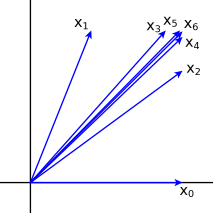
\includegraphics{4_e_Power_Method_1}}
\end{center}
\caption{The power method.}
\label{F:4_e_1}
\end{figure}
This method of successive approximations $\vx_k = A \vx_{k-1}$ is called the \emph{power method}\index{power method} (since we could write $\vx_k$ as $A^k \vx_0$). Our task now is to show that this method works in general. In the next activity we restrict our argument to the $2 \times 2$ case, and then discuss the general case afterwards. 



Let $A$ be an arbitrary $2 \times 2$ matrix with two linearly independent eigenvectors $\vv_1$ and $\vv_2$ and corresponding eigenvalues $\lambda_1$ and $\lambda_2$, respectively. We will also assume $|\lambda_1| > |\lambda_2|$. An eigenvalue  whose absolute value is larger than that of any other eigenvalue is called a \emph{dominant eigenvalue}\index{dominant eigenvalue}. Any eigenvector for a dominant eigenvalue is called a \emph{dominant eigenvector}\index{dominant eigenvector}. Before we show that our method can be used to approximate a dominant eigenvector, we recall that since $\vv_1$ and $\vv_2$ are eigenvectors corresponding to distinct eigenvalues, then $\vv_1$ and $\vv_2$ are linearly independent. So there exist scalars $a_1$ and $a_2$ such that 
\[\vx_0 = a_1 \vv_1 + a_2 \vv_2.\]
We have seen that for each positive integer $k$ we can write $\vx_n$ as 
\begin{equation} \label{eq:4_e_1}
\vx_k = a_1 \lambda_1^k \vv_1 + a_2 \lambda_2^k \vv_2. 
\end{equation}
With this representation of $\vx_0$ we can now see why the power method approximates a dominant eigenvector of $A$. 



\begin{activity} \label{act:4_e_1} Assume as above that $A$ is an arbitrary $2 \times 2$ matrix with two linearly independent eigenvectors $\vv_1$ and $\vv_2$ and corresponding eigenvalues $\lambda_1$ and $\lambda_2$, respectively. (We are assuming that we don't know these eigenvectors, but we can assume that they exist.) Assume that $\lambda_1$ is the dominant eigenvalue for $A$, $\vx_0$ is some initial guess to an eigenvector for $A$, that $\vx_0 = a_1 \vv_1 + a_2 \vv_2$, and that $\vx_k = A\vx_{k-1}$ for $k \geq 1$.
	\ba
	\item We divide both sides of equation (\ref{eq:4_e_1}) by $\lambda_1^k$ (since $\lambda_1$ is the dominant eigenvalue, we know that $\lambda_1$ is not $0$) to obtain
\begin{equation} \label{eq:4_e_2}
\frac{1}{\lambda_1^k}\vx_k = a_1 \vv_1 + a_2 \left(\frac{\lambda_2}{\lambda_1}\right)^k \vv_2.
\end{equation} 
Recall that $\lambda_1$ is the dominant eigenvalue for $A$. What happens to $\left( \frac{\lambda_2}{\lambda_1} \right)^k$ as $k \to \infty$? Explain what happens to the right hand side of equation (\ref{eq:4_e_2}) as $k \to \infty$.
	
	
	
	\item Explain why the previous result tells us that the vectors $\vx_k$ are approaching a vector in the \emph{direction} of $\vv_1$ or $-\vv_1$ as $k \to \infty$, assuming $a_1 \neq 0$. (Why do we need $a_1 \neq 0$? What happens if $a_1=0$?)

	
	
	\item What does all of this tell us about the sequence $\{\vx_k\}$ as $k \to \infty$?
	
	
	
	
	\ea
\end{activity}



The power method is straightforward to implement, but it is not without its drawbacks. We began by assuming that we had a basis of eigenvectors of a matrix $A$. So we are also assuming that $A$ is diagonalizable. We also assumed that $A$ had a dominant eigenvalue $\lambda_1$. That is, if $A$ is $n \times n$ we assume that $A$ has eigenvalues $\lambda_1$, $\lambda_2$, $\ldots$, $\lambda_n$, not necessarily distinct, with 
\[|\lambda_1| > |\lambda_2| \geq |\lambda_3| \geq \cdots \geq |\lambda_n|\]
and with $\vv_i$ an eigenvector of $A$ with eigenvalue $\lambda_i$. We could then write any initial guess $\vx_0$ in the form 
\[\vx_0 = a_1 \vv_1 +  a_2\vv_2 + \cdots + a_n \vv_n.\]
The initial guess is also called a \emph{seed}. 

Then 
\[\vx_k = a_1 \lambda_1^k \vv_1 + a_2 \lambda_2^k \vv_2 + \cdots + a_n \lambda_n^k \vv_n\]
 and
\begin{equation} \label{eq:4_e_3} 
\frac{1}{\lambda_1^k} \vx_k = a_1 \vv_1 + a_2 \left(\frac{\lambda_2}{\lambda_1}\right)^k \vv_2 + \cdots + a_n \left(\frac{\lambda_n}{\lambda_1}\right)^k \vv_n.
\end{equation} 
Notice that we are not actually calculating the vectors $\vx_k$ here -- this is a theoretical argument and we don't know $\lambda_1$ and are not performing any scaling like we did in Preview Activity \ref{pa:4_d}. We are assuming that $\lambda_1$ is the dominant eigenvalue of $A$, though, so for each $i$ the terms $\left(\frac{\lambda_i}{\lambda_1}\right)^k$ converge to $0$ as $k$ goes to infinity. Thus, 
\[\vx_k \approx \lambda_1^k a_1 \vv_1\]
 for large values of $k$, which makes the sequence $\{\vx_k\}$ converge to a vector in the direction of a dominant eigenvector $\vv_1$ provided $a_1 \neq 0$. So we need to be careful enough to choose a seed that has a nonzero component in the direction of $\vv_1$. Of course, we generally don't know that our matrix is diagonalizable before we make these calculations, but for many matrices the sequence $\{\vx_k\}$ will approach a dominant eigenvector. 
 
The power method approximates a dominant eigenvector, and there are ways that we can approximate the dominant eigenvalue. Exercise \ref{ex:4_d_dominant_eigenvalue} presents one way -- by keeping track of the components of the $\vx_k$ that have the largest absolute values, and the next activity shows another. 
 
 \begin{activity} \label{act:4_d_Rayleigh} Let $A$ be an $n \times n$ matrix with eigenvalue $\lambda$ and corresponding eigenvector $\vv$. 
 \ba
 \item Explain why $\lambda = \frac{\lambda (\vv \cdot \vv)}{\vv \cdot \vv}$. 
 
\item Use the result of part (a) to explain why $\lambda = \frac{(A\vv) \cdot \vv}{\vv \cdot \vv}$. 


\ea

\end{activity}

The result of Activity \ref{act:4_d_Rayleigh} is that, when the vectors in the sequence $\{\vx_k\}$  approximate a dominant eigenvector of a matrix $A$, the quotients
\begin{equation} \label{eq:Rayleigh}
\frac{(A\vx_k) \cdot \vx_k}{\vx_k \cdot \vx_k} = \frac{\vx_k^{\tr}A\vx_k}{\vx_k^{\tr}\vx_k}
\end{equation}
approximate the dominant eigenvalue of $A$. The quotients in (\ref{eq:Rayleigh}) are called \emph{Rayleigh quotients}\index{Rayleigh quotients}. 

 
To summarize, the procedure for applying the power method for approximating a dominant eigenvector and dominant eigenvalue of a matrix $A$ is as follows.
\begin{description}
\item[Step 1:] Select an arbitrary nonzero vector $\vx_0$ as an initial guess to a dominant eigenvector.
\item[Step 2:] Let $\vx_1 = A\vx_0$. Let $k = 1$. 
\item[Step 3:] To avoid having the magnitudes of successive approximations become excessively large, scale this approximation $\vx_k$. That is, find the entry $\alpha_k$ of $\vx_k$ that is largest in absolute value. Then replace $\vx_k$ by $\frac{1}{\alpha_k} \vx_k$.  
\item[Step 4:] Calculate the Rayleigh quotient $r_k = \frac{(A\vx_{k}) \cdot \vx_k}{\vx_k \cdot \vx_k}$.
\item[Step 5:] Let let $\vx_{k+1} = A \vx_k$. Increase $k$ by $1$ and repeat Steps 3 through 5.
\end{description}
If the sequence $\{\vx_k\}$ converges to a dominant eigenvector of $A$, then the sequence $\{r_k\}$ converges to the dominant eigenvalue of $A$. 

The power method can be useful for approximating a dominant eigenvector as long as the successive multiplications by $A$ are fairly simple -- for example, if many entries of $A$ are zero.\footnote{A matrix in which most entries are zero is called a \emph{sparse} matrix.\index{matrix!sparse}} The rate of convergence of the sequence $\{\vx_k\}$ depends on the ratio $\frac{\lambda_2}{\lambda_1}$. If this ratio is close to $1$, then it can take many iterations before the power $\left(\frac{\lambda_2}{\lambda_1}\right)^k$ makes the $\vv_2$ term negligible. There are other methods for approximating eigenvalues and eigenvectors, e.g., the QR factorization, that we will not discuss at this point.   	

\csection{The Inverse Power Method}
\label{sec:power_method_inv}

The power method only allows us to approximate the dominant eigenvalue and a dominant eigenvector for a matrix $A$. It is possible to modify this method to approximate other eigenvectors and eigenvalues under certain conditions. We consider an example in the next activity to motivate the general situation.



\begin{activity} \label{act:4_e_2} Let $A = \left[ \begin{array}{cc} 2&6 \\ 5&3 \end{array} \right]$ be the matrix from Preview Activity \ref{pa:4_d}. Recall that $8$ is an eigenvalue for $A$, and a quick calculation can show that $-3$ is the other eigenvalue of $A$. Consider the matrix $B = (A - (-2)I_2)^{-1} = \frac{1}{10}\left[ \begin{array}{rr} -5&6 \\ 5&-4 \end{array} \right]$. 
	\ba
	\item Show that $\frac{1}{8-(-2)}$ and $\frac{1}{-3-(-2)}$ are the eigenvalues of $B$. 



	\item Recall that $\vv_1 = [1 \ 1]^{\tr}$ is an eigenvector of $A$ corresponding to the eigenvalue $8$ and assume that $\vv_2 = [-6 \ 5]^{\tr}$ is an eigenvector for $A$ corresponding to the eigenvalue $-3$. Calculate the products $B \vv_1$ and $B \vv_2$. How do the products relate to the results of part (a)? 



	\ea
	
\end{activity}



Activity \ref{act:4_e_2} provides evidence that we can translate the matrix $A$ having a dominant eigenvalue to a different matrix $B$ with the same eigenvectors as $A$ and with a dominant eigenvalue of our choosing. To see why, let $A$ be an $n \times n$ matrix with eigenvalues $\lambda_1$, $\lambda_2$, $\ldots$, $\lambda_n$, and let $\alpha$ be any real number distinct from the eigenvalues. Let $B = (A - \alpha I_n)^{-1}$. In our example in Activity \ref{act:4_e_2} the numbers 
\[\frac{1}{\lambda_1 - \alpha}, \  \frac{1}{\lambda_2 - \alpha}, \ \frac{1}{\lambda_3 - \alpha}, \ \ldots, \frac{1}{\lambda_n - \alpha}\]
were the eigenvalues of $B$, and that if $\vv_i$ is an eigenvector for $A$ corresponding to the eigenvalue $\lambda_i$, then $\vv_i$ is an eigenvector of $B$ corresponding to the eigenvalue $\frac{1}{\lambda_i - \alpha}$. To see why, let $\lambda$ be an eigenvalue of an $n \times n$ matrix $A$ with corresponding eigenvector $\vv$. Let $\alpha$ be a scalar that is not an eigenvalue of $A$, and let $B = (A - \alpha I_n)^{-1}$. Now 
\begin{align*}
A \vv &= \lambda \vv \\
A \vv - \alpha \vv &= \lambda \vv - \alpha \vv \\
(A-\alpha I_n) \vv &= (\lambda - \alpha) \vv \\
\frac{1}{\lambda - \alpha} \vv &= (A-\alpha I_n)^{-1} \vv.
\end{align*}
So $\frac{1}{\lambda - \alpha}$ is an eigenvalue of $B$ with eigenvector $\vv$. 

Now suppose that $A$ is an $n \times n$ matrix with eigenvalues $\lambda_1$, $\lambda_2$, $\ldots$, $\lambda_n$, and that we want to approximate an eigenvector and corresponding eigenvalue $\lambda_i$ of $A$. If we can somehow find a value of $\alpha$ so that $|\lambda_i - \alpha| < |\lambda_j - \alpha|$ for all $j \neq i$, then $\left| \frac{1}{\lambda_i - \alpha} \right| > \left| \frac{1}{\lambda_j - \alpha} \right|$ for any $j \neq i$. Thus, the matrix $B = (A - \alpha I_n)^{-1}$ has $\frac{1}{\lambda_i - \alpha}$ as its dominant eigenvalue and we can use the power method to approximate an eigenvector and the Rayleigh quotient to approximate the eigenvalue $\frac{1}{\lambda_i - \alpha}$, and hence approximate $\lambda_i$.  



\begin{activity} \label{act:4_e_3} Let $A = \frac{1}{8}\left[ \begin{array}{crr} 7&3&3 \\ 30&22&-10 \\ 15&-21&11 \end{array} \right]$. 
	\ba
	\item Apply the power method to the matrix $B = (A - I_3)^{-1}$ with initial vector $\vx_0 = [1 \ 0 \ 0]^{\tr}$ to fill in Table \ref{T:4_e_2} (to four decimal places). Use this information to estimate an eigenvalue for $A$ and a corresponding eigenvector. 
\begin{table}[h]
\begin{center}
\renewcommand{\arraystretch}{2.0}
\begin{tabular}{cccc} 
$k$												&$10$		&$15$		&$20$		 \\ \hline
$\vx_k$											&\hspace{1.0in}	&\hspace{1.0in}	&\hspace{1.0in}		\\ \hline
$\frac{\vx_k^{\tr}A\vx_k}{\vx_k^{\tr}\vx_k}$ 	&	&	&		\\ \hline
\end{tabular}
\caption{Applying the power method to $(A - I_3)^{-1}$.}
\label{T:4_e_2}
\end{center}
\end{table}



	\item Applying the power method to the matrix $B = (A - 0I_3)^{-1}$ with initial vector $\vx_0 = [1 \ 0 \ 0]^{\tr}$ yields the information in Table \ref{T:4_e_3} (to four decimal places). Use this information to estimate an eigenvalue for $A$ and a corresponding eigenvector. 

\begin{table}[h]
\begin{center}
\renewcommand{\arraystretch}{2.0}
\begin{tabular}{cccc} \hline
$k$			&$10$		&$15$		&$20$		 \\ \hline %&$25$
$\vx_k$		&$\left[ \begin{array}{r} -0.3344 \\ 0.6677 \\ 1.0000 \end{array} \right]$	&$\left[\begin{array}{r} -0.3333 \\ 0.6666 \\ 1.0000 \end{array} \right]$	&$\left[ \begin{array}{r} -0.3333 \\ 0.6666 \\ 1.0000 \end{array} \right]$		\\ \hline %&$[-0.3333 \ 0.6666 \ 1.0000]^{\tr}$
$\frac{\vx_k^{\tr}A\vx_k}{\vx_k^{\tr}\vx_k}$ 	&$-1.0014$	&$-1.0000$	&$-1.0000$		\\ \hline %&$-1.0000$
\end{tabular}
\caption{Applying the power method to $(A - 0I_3)^{-1}$.}
\label{T:4_e_3}
\end{center}
\end{table}


%Eigenvector $[1/3 \ -2/3 \ -1]^{\tr}$ with eigenvalue $\lambda$ satisfying $\frac{1}{\lambda-0} = -1$ or $\lambda = -1$.



	\item Applying the power method to the matrix $B = (A - 5I_3)^{-1}$ with initial vector $\vx_0 = [1 \ 0 \ 0]^{\tr}$ yields the information in Table \ref{T:4_e_4} (to four decimal places). Use this information to estimate an eigenvalue for $A$ and a corresponding eigenvector. 

\begin{table}[h]
\begin{center}
\renewcommand{\arraystretch}{2.0}
\begin{tabular}{cccc} \hline
$k$			&$10$		&$15$		&$20$		\\ \hline %&$25$ 
$\vx_k$		&$\left[ \begin{array}{r} 0.0000 \\ 1.0000 \\ -1.0000 \end{array} \right]$	&$\left[ \begin{array}{r} 0.0000 \\ 1.0000 \\ -1.0000 \end{array} \right]$	&$\left[ \begin{array}{r} 0.0000 \\ 1.0000 \\ -1.0000 \end{array} \right]$		\\ \hline %&$[0.0000 \ -1.0000 \ 1.0000]^{\tr}$
$\frac{\vx_k^{\tr}A\vx_k}{\vx_k^{\tr}\vx_k}$ 	&$-1.0000$	&$-1.0000$	&$-1.0000$		\\ \hline %&$-1.0000$
\end{tabular}
\caption{Applying the power method to $(A - 5I_3)^{-1}$.}
\label{T:4_e_4}
\end{center}
\end{table}

%Eigenvector $[0 \ 1 \ -1]^{\tr}$ with eigenvalue $\lambda$ satisfying $\frac{1}{\lambda-5} = -1$ or $\lambda = 4$.



	\ea
	
\end{activity}

\csection{Examples}
\label{sec:app_eigen_exam}
\ExampleIntro

\begin{example} Let $A = \left[ \begin{array}{ccc} 1&2&3\\4&5&6\\7&8&9 \end{array} \right]$.
\ba
\item Approximate the dominant eigenvalue of $A$ accurate to two decimal places using the power method. Use technology as appropriate.

\item Find the characteristic polynomial $p(\lambda)$ of $A$. Then find the the root of $p(\lambda)$ farthest from the origin. Compare to the result of part (a). Use technology as appropriate.

\ea

\ExampleSolution
\ba
\item We use technology to calculate the scaled vectors $A^k \vx_0$ for values of $k$ until the components don't change in the second decimal place. We start with the seed $\vx_0 = [1 \ 1 \ 1]^{\tr}$. For example, to two decimal places we have $\vx_k = [0.28 \ 0.64 \ 1.00]^{\tr}$ for $k  \geq 20$. So we suspect that $\left[ 0.28 \ 0.64 \ 1.00 \right]^{\tr}$ is close to a dominant eigenvector for $A$. 

For the dominant eigenvalue, we can calculate the Rayleigh quotients $\frac{(A\vx_k) \cdot \vx_k}{\vx_k \cdot \vx_k}$ until they do not change to two decimal places. For $k \geq 4$, our Rayleigh quotients are all (to two decimal places) equal to $16.12$. So we expect that the dominant eigenvalue of $A$ is close to $16.12$. Notice that 
\[A [0.28 \ 0.64 \ 1.00]^{\tr} =  [4.56 \ 10.32 \ 16.08]^{\tr},\]
which is not far off from $16.12 [0.28 \ 0.64 \ 1.00]^{\tr}$. 

\item The characteristic polynomial of $A$ is 
\[p(\lambda) =-\lambda^3 + 15 \lambda^2 + 18 \lambda = -\lambda(\lambda^2-15\lambda-18).\]
The quadratic formula gives the nonzero roots of $p(\lambda)$ as 
\[\frac{15 \pm \sqrt{15^2 + 4(18)}}{2} = \frac{15 \pm 3\sqrt{33}}{2}.\]
The roots farthest from the origin is approximately $16.12$, as was also calculated in part (a).  
\ea

\end{example}


\begin{example} Let $A = \left[ \begin{array}{ccc} 2&1&0 \\ 1&3&1 \\ 0&1&2 \end{array} \right]$.
\ba
\item Use the power method to approximate the dominant eigenvalue and a corresponding eigenvector (using scaling) accurate to two decimal places. Use $\vx_0 = [1 \ 1 \ 1]^{\tr}$ as the seed.

\item Determine the exact value of the dominant eigenvalue of $A$ and compare to your result from part (a).

\item Approximate the remaining eigenvalues of $A$ using the inverse power method. (Hint: Try $\alpha = 0.5$ and $\alpha = 1.8$.)

\ea

\ExampleSolution
\ba
\item We use technology to calculate the scaled vectors $A^k \vx_0$ for values of $k$ until the components don't change in the second decimal place. For example, to two decimal places we have $\vx_k = [0.50 \ 1.00 \ 0.50]^{\tr}$ for $k \geq 4$. So we suspect that $\left[ \frac{1}{2} \ 1 \ \frac{1}{2} \right]^{\tr}$ is a dominant eigenvector for $A$. 

For the dominant eigenvalue, we can calculate the Rayleigh quotients $\frac{(A\vx_k) \cdot \vx_k}{\vx_k \cdot \vx_k}$ until they do not change to two decimal places. For $k \geq 2$, our Rayleigh quotients are all (to two decimal places) equal to $4$. So we expect that the dominant eigenvalue of $A$ is $4$. We could also use the fact that 
\[A \left[ \frac{1}{2} \ 1 \ \frac{1}{2} \right]^{\tr} = [2 \ 4 \ 2]^{\tr} = 4\left[ \frac{1}{2} \ 1 \ \frac{1}{2} \right]^{\tr} \]
to see that $\left[ \frac{1}{2} \ 1 \ \frac{1}{2} \right]^{\tr}$ is a dominant eigenvector for $A$ with eigenvalue $4$. 

\item Technology shows that the characteristic polynomial of $A - \lambda I_3$ is 
\[p(\lambda) = -\lambda^3 + 7\lambda^2 - 14 \lambda + 8 = -(\lambda-1)(\lambda-2)(\lambda-4).\]
We can see from the characteristic polynomial that $4$ is the dominant eigenvalue of $A$. 

\item Applying the power method to $B = (A-0.5I_3)^{-1}$ with seed $\vx_0 = [1 \ 1 \ 1]^{\tr}$ gives $\vx_k \approx [ 0.50 \ 1.00 \ 0.50]^{\tr}$ for $k \geq 5$, with Rayleigh quotients of $2$ (to several decimal places). So $2$ is the dominant eigenvalue of $B$. But $\frac{1}{\lambda-0.5}$ is also the dominant eigenvalue of $B$, where $\lambda$ is the corresponding eigenvalue of $A$. . So to find $\lambda$, we note that $\frac{1}{\lambda-0.5} = 2$ implies that $\lambda = 1$ is an eigenvalue of $A$.  

Now applying the power method to $B = (A-1.8I_3)^{-1}$ with seed $\vx_0 = [1 \ 1 \ 1]^{\tr}$ gives $\vx_k \approx [ 1.00 \ -1.00 \ 1.00]^{\tr}$ for large enough $k$, with Rayleigh quotients of $5$ (to several decimal places). To find the corresponding eigenvalue $\lambda$ for $A$, we note that $\frac{1}{\lambda-1.8} = 5$, or  $\lambda = 2$ is an eigenvalue of $A$.  

Admittedly, this method is very limited. Finding good choices for $\alpha$ often depends on having some information about the eigenvalues of $A$. Choosing $\alpha$ close to an eigenvalue provides the best chance of obtaining that eigenvalue.   

\ea

\end{example}


\csection{Summary}
\label{sec:app_eigen_summ}
\begin{itemize}
\item The power method is an iterative method that can be used to approximate the dominant eigenvalue of an $n \times n$ matrix $A$ that has $n$ linearly independent eigenvectors and a dominant eigenvalue. 
\item To use the power method we start with a seed $\vx_0$ and then calculate the sequence $\{\vx_k\}$ of vectors, where $\vx_k = A \vx_{k-1}$. If $\vx_0$ is chosen well, then the sequence $\{\vx_k\}$ converges to a dominant eigenvector of $A$. 
\item If $A$ is an $n \times n$ matrix with eigenvalues $\lambda_1$, $\lambda_2$, $\ldots$, $\lambda_n$, to approximate an eigenvector of $A$ corresponding to the eigenvalue $\lambda_i$, we apply the power method to the matrix $B = (A - \alpha I_n)^{-1}$, where $\alpha$ is not a eigenvalue of $A$ and $\left| \frac{1}{\lambda_i - \alpha} \right| > \left| \frac{1}{\lambda_j - \alpha} \right|$ for any $j \neq i$. 
\end{itemize}

\csection{Exercises}
\label{sec:app_eigen_exer}

\be
\item Let $A = \left[ \begin{array}{cc} 1&2\\2&1 \end{array} \right]$. Let $\vx_0 = [1 \ 0]^{\tr}$. 
	\ba
	\item Find the eigenvalues and corresponding eigenvectors for $A$. 
	\item Use appropriate technology to calculate $\vx_k = A^k \vx_0$ for $k$ up to 10. Compare to a dominant eigenvector for $A$. 
	\item Use the eigenvectors from part (b) to approximate the dominant eigenvalue for $A$. Compare to the exact value of the dominant eigenvalue of $A$. 
	\item Assume that the other eigenvalue for $A$ is close to $0$. Apply the inverse power method and compare the results to the remaining eigenvalue and eigenvectors for $A$.
	\ea

\item Let $A = \left[ \begin{array}{rcc} 1&2&0\\-2&1&2 \\ 1&3&1 \end{array} \right]$. Use the power method to approximate a dominant eigenvector for $A$.  Use $\vx_0 = [1 \ 1 \ 1]^{\tr}$ as the seed. Then approximate the dominant eigenvalue of $A$. 

\item Let $A = \left[ \begin{array}{rr} 3&-1\\-1&3 \end{array} \right]$. Use the power method starting with $\vx_0 = [1 \ 1]^{\tr}$. Explain why the method fails in this case to approximate a dominant eigenvector, and how you could adjust the seed to make the process work.  

\item Let $A = \left[ \begin{array}{cc} 0&1\\1&0 \end{array} \right]$. 
	\ba
	\item Find the eigenvalues and an eigenvector for each eigenvalue.
	
	\item Apply the power method with an initial starting vector $\vx_0 = [0 \ 1]^{\tr}$. What is the resulting sequence? 
	
	\item Use equation (\ref{eq:4_e_3}) to explain the sequence you found in part (b).
	
	\ea


\item Let $A = \left[ \begin{array}{cc} 2&6 \\ 5&3 \end{array} \right]$. Fill in the entries in Table \ref{T:4_e_1}, where $\vx_k$ is the $k$th approximation to a dominant eigenvector using the power method, starting with the seed $\vx_0 = [1 \ 0]^{\tr}$. Compare the results of this table to the eigenvalues of $A$ and $\lim_{k \to \infty} \frac{\vx_{k+1}\cdot \vx_k}{\vx_k \cdot \vx_k}$. What do you notice? 

\begin{table}[h]
\begin{center}
\renewcommand{\arraystretch}{1.4}
\begin{tabular}{ccccccc} 
$\vv$ &$\vx_0$	&$\vx_1$	&$\vx_2$	&$\vx_3$	&$\vx_4$	&$\vx_5$ 		\\ 
$\frac{\vv^{\tr}A\vv}{\vv^{\tr}\vv}$ 	&\hspace{0.25in}	&\hspace{0.25in}	&\hspace{0.25in}	&\hspace{0.25in}	&\hspace{0.25in}	&\hspace{0.25in}		\\ \hline
\end{tabular}
\begin{tabular}{ccccccc} \hline
$\vv$ &$\vx_6$	&$\vx_7$	&$\vx_8$	&$\vx_9$	&$\vx_{10}$ &$\vx_{11}$	\\ 
$\frac{\vv^{\tr}A\vv}{\vv^{\tr}\vv}$ 	&\hspace{0.25in}	&\hspace{0.25in}	&\hspace{0.25in}	&\hspace{0.25in}	&\hspace{0.25in}	&\hspace{0.25in}		\\ 
\end{tabular}
\caption{Values of the Rayleigh quotient.}
\label{T:4_e_1}
\end{center}
\end{table}

\item Let $A = \left[ \begin{array}{cr} 4&-5 \\ 2&15 \end{array} \right]$. The power method will approximate the dominant eigenvalue $\lambda = 14$. In this exercise we explore what happens if we apply the power method to $A^{-1}$. 
\ba
\item Apply the power method to $A^{-1}$ to approximate the dominant eigenvalue of $A^{-1}$.  Use $[1 \ 1]^{\tr}$ as the seed. How is this eigenvalue related to an eigenvalue of $A$?

\item Explain in general why applying the power method to the inverse of an invertible matrix $B$ might give an approximation to an eigenvalue of $B$ of smallest magnitude. When might this not work? 

\ea


\item There are other algebraic methods that do not rely on the determinant of a matrix that can be used to find eigenvalues of a matrix. We examine one such method in this exercise. Let $A$ be any $n \times n$ matrix, and let $\vv$ be any vector in $\R^n$. 
	\ba
	\item Explain why the vectors  
\[\vv, \ A\vv, \ A^2\vv, \ \ldots, \ A^n\vv\]
are linearly dependent. 

	\item Let $c_0$, $c_1$, $\ldots$, $c_n$ be scalars, not all 0, so that  
\[c_0 \vv + c_1 A\vv + c_2 A^2 \vv + \cdots + c_n A^n \vv = \vzero.\]
Explain why there must be a smallest positive integer $k$ so that there are scalars $a_0$, $a_1$, $\ldots$, $a_k$ with $a_k \neq 0$. such that  
\[a_0 \vv + a_1 A\vv + a_2 A^2 \vv + \cdots + a_k A^k \vv = \vzero.\]

	\item Let 
\[q(t) = a_0 + a_1t + a_2t^2 + \cdots + a_kt^k.\]
Then
\[q(A) = a_0 + a_1A + a_2A^2 + \cdots + a_kA^k\]
and
\begin{align*}
q(A)\vv &= (a_0 + a_1A + a_2A^2 + \cdots + a_kA^k)\vv \\
	&= a_0 \vv + a_1 A\vv + a_2 A^2 \vv + \cdots + a_k A^k \vv \\
	&= \vzero.
\end{align*}
Suppose the polynomial $q(t)$ has a linear factor, say $q(t) = (t-\lambda)Q(t)$ for some degree $k-1$ polynomial $Q(t)$. Explain why, if $Q(A) \vv$ is non-zero,  $\lambda$ is an eigenvalue of $A$ with eigenvector $Q(A) \vv$. 

	\item This method allows us to find certain eigenvalues and eigenvectors, the roots of the polynomial $q(t)$. Any other eigenvector must lie outside the eigenspaces we have already found, so repeating the process with a vector $\vv$ not in any of the known eigenspaces will produce different eigenvalues and eigenvectors. Let $A = \left[ \begin{array}{ccr} 2&2&-1 \\ 2&2&2 \\ 0&0&6 \end{array} \right]$.
	\begin{enumerate}[i.]
	\item Find the polynomial $q(t)$. Use $\vv = [1 \ 1 \ 1]^{\tr}$.
	\item Find all of the roots of $q(t)$.
	\item For each root $\lambda$ of $q(t)$, find the polynomial $Q(t)$ and use this polynomial to determine an eigenvector of $A$. Verify your work.
	\end{enumerate}
	\ea

\item \label{ex:4_d_dominant_eigenvalue} We have seen that the Rayleigh quotients approximate the dominant eigenvalue of a matrix $A$. As an alternative to using Rayleigh quotients, we can keep track of the scaling factors. Recall that the scaling in the power method can be used to make the magnitudes of the successive approximations smaller and easier to work with. Let $A$ be an $n \times n$ matrix and begin with a non-zero seed $\vv_0$. We now want to keep track of the scaling factors, so let $\alpha_0$ be the component of $\vv_0$ with largest absolute value and let $\vx_0 = \frac{1}{\alpha_0}\vv_0$. For $k \geq 0$, let $\vv_k = A\vx_{k-1}$, let $\alpha_k$ be the component of $\vv_k$ with largest absolute value and let $\vx_k = \frac{1}{\alpha_k}\vv_k$. 
\ba
\item Let $A = \left[ \begin{array}{rc} 0&1 \\ -8&6 \end{array} \right]$. Use $\vx_0 = [1 \ 1]^{\tr}$ as the seed and calculate $\alpha_k$ for $k$ from $1$ to $10$. Compare to the dominant eigenvalue of $A$.

\item Assume that for large $k$ the vectors $\vx_k$ approach a dominant eigenvector with dominant eigenvalue $\lambda$. Show now in general that the sequence of scaling factors $\alpha_k$ approaches $\lambda$. 

\ea

\item Let $A$ be an $n \times n$ matrix and let $\alpha$ be a scalar that is not an eigenvalue of $A$. Suppose that $\vx$ is an eigenvector of $B = (A-\alpha I_n)^{-1}$ with eigenvalue $\beta$. Find an eigenvalue of $A$ in terms of $\beta$ and $\alpha$ with  corresponding eigenvector $\vx$.

	
\item Label each of the following statements as True or False. Provide justification for your response.
\ba
\item \textbf{True/False} The largest eigenvalue of a matrix is a dominant eigenvalue. 

\item \textbf{True/False} If an $n \times n$ matrix $A$ has $n$ linearly independent eigenvectors and a dominant eigenvalue, then the sequence $\{A^k \vx_0\}$ converges to a dominant eigenvector of $A$ for any initial vector $\vx_0$. 

\item \textbf{True/False} If $\lambda$ is an eigenvalue of an $n \times n$ matrix $A$ and $\alpha$ is not an eigenvalue of $A$, then $\lambda - \alpha$ is an eigenvalue of $A - \alpha I_n$. 

\item \textbf{True/False} Every square matrix has a dominant eigenvalue. 
\ea

\ee

\csection{Project: Managing a Sheep Herd}
\label{sec:proj_sheep_herd}

Sheep farming is a significant industry in New Zealand. New Zealand is reported to have the highest density of sheep in the world. Sheep can begin to reproduce after one year, and give birth only once per year. Table \ref{T:Sheep} gives Birth and Survival Rates for Female New Zealand Sheep (from G. Caughley, ``Parameters for Seasonally Breeding Populations," \emph{Ecology}, \textbf{48}, (1967), 834-839). Since sheep hardly ever live past 12 years, we will only consider the population through 12 years.
%\verb+http://www.math.uri.edu/~bonifant/classes/spring07/mth215/proj2.pdf+
\begin{table}[h]
\begin{center}
\begin{tabular}{| c | c | c |}  \hline
Age (years) &Birth Rate 	&Survival Rate \\ \hline
0-1 		&0.000 			&0.845 \\ \hline
1-2 		&0.045 			&0.975 \\ \hline
2-3 		&0.391 			&0.965 \\ \hline
3-4 		&0.472 			&0.950 \\ \hline
4-5 		&0.484 			&0.926 \\ \hline
5-6 		&0.546 			&0.895 \\ \hline
6-7 		&0.543 			&0.850 \\ \hline
7-8 		&0.502 			&0.786 \\ \hline
8-9 		&0.468 			&0.691 \\ \hline
9-10 		&0.459 			&0.561 \\ \hline
10-11 	&0.433 			&0.370 \\ \hline
11-12 	&0.421 			&0.000 \\ \hline
\end{tabular}
\caption{New Zealand female sheep data by age group.}
\label{T:Sheep}
\end{center}
\end{table}

As sheep reproduce, they add to the 0-1 sheep (lamb) population. The potential to produce offspring is called \emph{fecundity} (derived from the word \emph{fecund} which generally refers to reproductive ability) and determines how many lamb are added to the population. Let $F_k$ (the fecundity rate) be the rate at which females in age class $k$ give birth to female offspring. Not all members of a given age group survive to the next age groups, so let $s_k$ be the fraction of individuals that survives from age group $k$ to age group $k+1$. With these ideas  in mind, we can create a life cycle chart as in Figure \ref{F:Life_cycle} that illustrates how the population of sheep changes on a farm (for the sake of space, we illustrate with four age classes). 

\begin{figure}[ht]
\begin{center}
\resizebox{!}{1.5in}{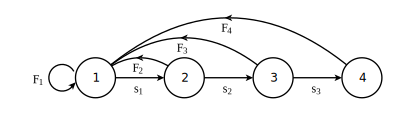
\includegraphics{4_d_Cycles}}
\caption{Life cycle with four age classes.}
\label{F:Life_cycle}
\end{center}
\end{figure}


\begin{comment}
\begin{figure}[ht]
\begin{center}
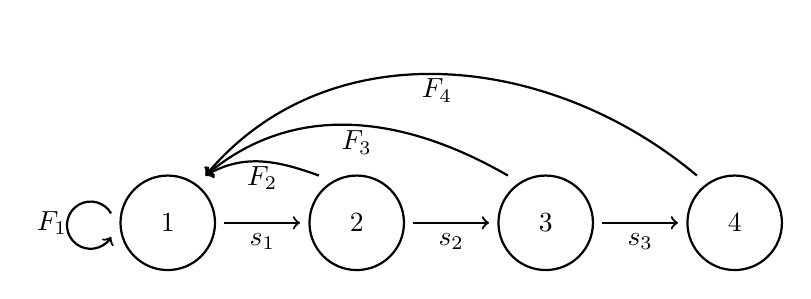
\begin{tikzpicture}[scale=0.6]
	\def\firstcircle{(0,0) circle (1cm)}
	\def\secondcircle{(4,0) circle (1cm)}
	\def\thirdcircle{(8,0) circle (1cm)}
	\def\fourthcircle{(12,0) circle (1cm)}
%	\draw (-4,-4.5) -- (4,-4.5) -- (4,2.75) -- (-4,2.75) -- cycle;
%	\begin{scope}
%	\clip \firstcircle;
%	\draw[fill=gray!30] \secondcircle;
%	\end{scope}
%	\draw[fill=gray!30] \thirdcircle;
	\draw[thick] \firstcircle;
	\draw[thick] \secondcircle;	
	\draw[thick] \thirdcircle;	
	\draw[thick] \fourthcircle;		
	\draw[->, thick](1.2,0) -- (2.8,0);
	\draw[->, thick](5.2,0) -- (6.8,0);
	\draw[->, thick](9.2,0) -- (10.8,0);
	%curve start point, end point, angle at start, angle at end
	\draw[->,thick] (3.2,1.0) to [out=160,in=30](0.8,1.0);
	\draw[->,thick] (7.2,1.0) to [out=150,in=40](0.8,1.0);
	\draw[->,thick] (11.2,1.0) to [out=140,in=50](0.8,1.0);
	\draw[thick] [->] (-1.2,0.2) arc (30:330:0.5); %center of arc, arc (start degree, end degree, radius) 
	\node at (0,0) {$1$};
	\node at (4,0) {$2$};
	\node at (8,0) {$3$};
	\node at (12,0) {$4$};
	\node at (2,-0.4) {$s_1$};
	\node at (6,-0.4) {$s_2$};
	\node at (10,-0.4) {$s_3$};
	\node at (-2.45,0.0) {$F_1$};
	\node at (2,0.95) {$F_2$};
	\node at (4,1.7) {$F_3$};
	\node at (5.7,2.8) {$F_4$};
\end{tikzpicture}
\caption{Life cycle with four age classes.}
\label{F:Life_cycle}
\end{center}
\end{figure}
\end{comment}

To model the sheep population, we need a few variables. Let $n_1^{(0)}$ be the number of sheep in age group 0-1, $n_2^{(0)}$ the number in age group 1-2, $n_3$ the number in age group 2-3 and, in general, $n_k^{(0)}$ the number of sheep in age group $(k-1)$-$k$ at some initial time (time $0$), and let 
\[\vx_0 = \left[ n_1^{(0)} \ n_2^{(0)} \ n_3^{(0)} \ \cdots \ n_{12}^{(0)} \right]^{\tr}.\]
We wish to determine the populations in the different groups after one year. Let 
\[\vx_1 = \left[ n_1^{(1)} \ n_2^{(1)} \ n_3^{(1)}  \ \cdots \ n_{12}^{(1)} \right]^{\tr},\]
where $n_1^{(1)}$ denotes the number of sheep in age group 0-1, $n_2^{(1)}$ the number of sheep in age group 1-2 and, in general, $n_{k}^{(1)}$ the number of tilapia in age group $(k-1)$-$k$ after one year. 

\begin{pactivity} \label{Leslie_1} Table \ref{T:Sheep} shows that, on average, each female in age group 1-2 produces $0.045$ female offspring in a year. Since there are $n_2$ females in age group 1-2, the lamb population increases by $0.045n_2$ in a year. 
	\ba
	\item Continue this analysis to explain why 
	\begin{align*}
	n_1^{(1)} &= 0.045n_2+0.391 n_3+0.472n_4+0.484 n_5+0.546n_6+0.543n_7 \\
		&\qquad+0.502 n_8+0.468 n_9+0.459n_{10}+0.433 n_{11}+0.421 n_{12}.
	\end{align*}
	
	\item Explain why $n_2^{(1)} = 0.845n_1$. 
	
	\item Now explain why 
\begin{equation}
\vx_1 = L\vx_0, \label{eq:Leslie_1}
\end{equation}
where $L$ is the matrix 
 \begin{equation} \label{eq:Leslie_2}
 {\scriptsize \hspace*{-0.25in} \left[\arraycolsep=2.0pt  \begin{array}{cccccccccccc} 
0     	& 0.045 & 0.391 & 0.472 & 0.484 & 0.546 & 0.543 & 0.502 & 0.468 & 0.459 & 0.433 & 0.421 \\
0.845 	& 0 	& 0 	& 0 	& 0 	& 0 	& 0 	& 0 	& 0 	& 0 	& 0 	& 0 \\
0 		& 0.975 & 0		& 0 	& 0 	& 0 	& 0 	& 0 	& 0 	& 0 	& 0 	& 0 \\
0 		& 0 	& 0.965	& 0 	& 0 	& 0 	& 0 	& 0 	& 0 	& 0 	& 0 	& 0 \\
0 		& 0 	& 0		& 0.950	& 0 	& 0 	& 0 	& 0 	& 0 	& 0 	& 0 	& 0 \\
0 		& 0 	& 0		& 0		& 0.926 & 0 	& 0 	& 0 	& 0 	& 0 	& 0 	& 0 \\
0 		& 0 	& 0		& 0		& 0 	& 0.895	& 0 	& 0 	& 0 	& 0 	& 0 	& 0 \\
0 		& 0 	& 0		& 0		& 0 	& 0		& 0.850	& 0 	& 0 	& 0 	& 0 	& 0 \\
0 		& 0 	& 0		& 0		& 0 	& 0		& 0		& 0.786	& 0 	& 0 	& 0 	& 0 \\
0 		& 0 	& 0		& 0		& 0 	& 0		& 0		& 0		& 0.691	& 0 	& 0 	& 0 \\
0 		& 0 	& 0		& 0		& 0 	& 0		& 0		& 0		& 0		& 0.561	& 0 	& 0 \\
0 		& 0 	& 0		& 0		& 0 	& 0		& 0		& 0		& 0		& 0		& 0.370	& 0 \\
\end{array} \right]}.
\end{equation}

	\ea
\end{pactivity}

Notice that our matrix $L$ has the form 
\[\left[ \begin{array}{cccccc} F_1&F_2&F_3&\cdots&F_{n-1}&F_n \\ s_1&0&0&\cdots&0&0 \\ 0&s_2&0&\cdots&0&0 \\  0&0&s_3&\cdots&0&0 \\ &&&\ddots&& \\ 0&0&0&\cdots&s_{n-1}&0 \end{array} \right].\]
Such a matrix is called a \emph{Leslie matrix}\index{Leslie matrix}\index{Leslie matrix}. 

Leslie matrices have certain useful properties, and one eigenvalue of a Leslie matrix can tell us a lot about the long-term behavior of the situation being modeled. You can take these properties as fact unless otherwise directed.
\begin{enumerate}
\item A Leslie matrix $L$ has a unique positive eigenvalue $\lambda_1$ with a corresponding eigenvector $\vv_1$ whose entries are all positive.

\item If $\lambda_i$ ($i > 1$) is any other eigenvalue (real or complex) of $L$, then $|\lambda_i| \leq \lambda_1$. If $\lambda_1$ is the largest magnitude eigenvalue of a matrix $L$, we call $\lambda_1$ a \emph{dominant eigenvalue} of $L$.

\item If any two successive entries in the first row of $L$ are both positive, then $|\lambda_i| < \lambda_1$ for every $i > 1$. In this case we say that $\lambda_1$ is a \emph{strictly dominant eigenvalue} of $L$. In a Leslie model, this happens when the females in two successive age classes are fertile, which is almost always the case.

\item If $\lambda_1$ is a strictly dominant eigenvalue, then $\vx_k$ is approximately a scalar multiple of $\vv_1$ for large values of $k$, regardless of the initial state $\vx_0$. In other words, large state vectors are close to eigenvectors for $\lambda_1$.
\end{enumerate}

We can use these properties to determine the long-term behavior of the sheep herd.

\begin{pactivity} \label{act:Leslie_2} Assume that $L$ is defined by (\ref{eq:Leslie_2}), and let 
\[\vx_m = \left[ n_1^{(m)} \ n_2^{(m)} \ n_3^{(m)} \ \cdots \ n_{12}^{(m)} \right]^{\tr},\]
 where $n_1^{(m)}$ denotes the number of sheep in age group 0-1, $n_2^{(m)}$ the number of sheep in age group 1-2 and, in general, $n_k^{(m)}$ the number of sheep in age group $(k-1)$-$k$ after $k$ years. 
 	\ba
	 \item Assume that $\vx_0 = \left[100 \ 100 \ 100 \ \cdots \ 100  \right]^{\tr}$. Use appropriate technology to calculate $\vx_{22}$, $\vx_{23}$, $\vx_{24}$, and $\vx_{25}$. Round to the nearest whole number. What do you notice about the sheep population?  You may use the GeoGebra applet at \url{https://www.geogebra.org/m/yqss88xq}. 

	\item  We can use the third and fourth properties of Leslie matrices to better understand the long-term behavior of the sheep population. Since successive entries in the first row of the Leslie matrix in (\ref{eq:Leslie_2}) are positive, our Leslie matrix has a strictly dominant eigenvalue $\lambda_1$. Given the dimensions of our Leslie matrix, finding this dominant eigenvalue through algebraic means is not feasible. Use the power method to approximate the dominant eigenvalue $\lambda_1$ of the Leslie matrix in (\ref{eq:Leslie_2}) to five decimal places. Explain your process. Then explain how this dominant eigenvalue tells us that, unchecked, the sheep population grows at a rate that is roughly exponential. What is the growth rate of this exponential growth?  You may use the GeoGebra applet at \url{https://www.geogebra.org/m/yqss88xq}. 

	\ea

\end{pactivity}


Project Activity \ref{act:Leslie_2} indicates that, unchecked, the sheep population will grow without bound, roughly exponentially with ratio equal to the dominant eigenvalue of our Leslie matrix $L$. Of course, a sheep farmer cannot provide the physical environment or the resources to support an unlimited population of sheep. In addition, most sheep farmers cannot support themselves only by shearing sheep for the wool. Consequently, some harvesting of the sheep population each year for meat and skin is necessary. A sustainable harvesting policy allows for the regular harvesting of some sheep while maintaining the population at a stable level. It is necessary for the farmer to find an optimal harvesting rate to attain this stable population and the following activity leads us through an analysis of how such a harvesting rate can be determined.

\begin{pactivity} \label{act:Leslie_harvest} The Leslie model can be modified to consider harvesting. It is possible to harvest different age groups at different rates, and to harvest only some age groups and not others. In the case of sheep, it might make sense to only harvest from the youngest population since lamb is more desirable than mutton and the lamb population grows the fastest. Assume that this is our harvesting strategy and that we harvest our sheep from only the youngest age group at the start of each year. Let $h$ be the fraction of sheep we harvest from the youngest age group each year after considering growth.
\ba
\item If we begin with an initial population $\vx_0$, then the state vector after births and expected deaths is $L\vx_0$. Now we harvest. Explain why if we harvest a fraction $h$ from the youngest age group after considering growth, then the state vector after 1 year will be
\begin{equation*}
\vx_1 = L\vx_0 - HL\vx_0,
\end{equation*}
where
\[H =  \left[
\begin{array}{c c c c c c c c c c c c}
h    	& 0 	& 0 	& 0 	& 0 	& 0 	& 0 	& 0	 	& 0 	& 0 	& 0 	& 0 \\
0 		& 0 	& 0 	& 0 	& 0 	& 0 	& 0 	& 0 	& 0 	& 0 	& 0 	& 0 \\
0 		& 0 	& 0		& 0 	& 0 	& 0 	& 0 	& 0 	& 0 	& 0 	& 0 	& 0 \\
0 		& 0 	& 0		& 0 	& 0 	& 0 	& 0 	& 0 	& 0 	& 0 	& 0 	& 0 \\
0 		& 0 	& 0		& 0		& 0 	& 0 	& 0 	& 0 	& 0 	& 0 	& 0 	& 0 \\
0 		& 0 	& 0		& 0		& 0 	& 0 	& 0 	& 0 	& 0 	& 0 	& 0 	& 0 \\
0 		& 0 	& 0		& 0		& 0 	& 0		& 0 	& 0 	& 0 	& 0 	& 0 	& 0 \\
0 		& 0 	& 0		& 0		& 0 	& 0		& 0		& 0 	& 0 	& 0 	& 0 	& 0 \\
0 		& 0 	& 0		& 0		& 0 	& 0		& 0		& 0		& 0 	& 0 	& 0 	& 0 \\
0 		& 0 	& 0		& 0		& 0 	& 0		& 0		& 0		& 0		& 0 	& 0 	& 0 \\
0 		& 0 	& 0		& 0		& 0 	& 0		& 0		& 0		& 0		& 0		& 0 	& 0 \\
0 		& 0 	& 0		& 0		& 0 	& 0		& 0		& 0		& 0		& 0		& 0		& 0 \\
\end{array} \right].\]


\item Our goal is to find a harvesting rate that will lead to a steady state in which the sheep population remains the same each year. In other words, we want to find a value of $h$, if one exists, that satisfies
\begin{equation}
\vx = L\vx - HL\vx. \label{eq:Harvest}
\end{equation}
Show that (\ref{eq:Harvest}) is equivalent to the matrix equation
\begin{equation}
\vx = (I_{12}-H)L\vx. \label{eq:Harvest2}
\end{equation}

\item Use appropriate technology to experiment numerically with different values of $h$ to find the value you think gives the best uniform harvest rate. Explain your reasoning. You may use the GeoGebra applet at \url{https://www.geogebra.org/m/yqss88xq}. 


\item Now we will use some algebra to find an equation that explicitly gives us the harvest rate in the general setting. This will take a bit of work, but none of it is too difficult. To simplify our work but yet illustrate the overall idea, let us consider the general $4 \times 4$ case with arbitrary Leslie matrix
\begin{equation*} 
L = \left[ \begin{array}{cccc}
F_1 & F_2 	& F_3 	& F_4 \\
s_1 & 0 	& 0 	& 0  \\
0 	& s_2 	& 0 	& 0 \\
0 	& 0 	& s_3	& 0  \\
\end{array} \right].
\end{equation*}
Recall that we want to find a value of $h$ that satisfies (\ref{eq:Harvest2}) with $H = \left[ \begin{array}{cccc}
h   & 0 	& 0 	& 0 \\
0   & 0 	& 0 	& 0  \\
0 	& 0 	& 0 	& 0 \\
0 	& 0 	& 0	    & 0  \\
\end{array} \right].$
Let $\vx = [x_1 \  x_2 \ x_3 \ x_4]^{\tr}$.
        \begin{enumerate}[i.]
        \item Calculate the matrix product $(I_{4}-H)L$. Explain why this product is again a Leslie matrix and why $(I_{4}-H)L$ will have a dominant eigenvalue of 1.


        \item Now calculate $(I_{4}-H)L\vx$ and set it equal to $\vx$. Write down the resulting system of 4 equations that must be satisfied. Be sure that your first equation is
\begin{equation}
x_1 = (1-h)F_1x_1 + (1-h)F_2x_2 + (1-h)F_3x_3 + (1-h)F_4x_4. \label{eq:harvestval1}
\end{equation}

        \item Equation (\ref{eq:harvestval1}) as written depends on the entries of the vector $\vx$, but we should be able to arrive at a result that is independent of $\vx$. To see how we do this, we assume the population of the youngest group is never 0, so we can divide both sides of (\ref{eq:harvestval1}) by $x_1$ to obtain
\begin{equation} 
1 = (1-h)F_1 + (1-h)F_2 \frac{x_2}{x_1} + (1-h)F_3 \frac{x_3}{x_1} + (1-h)F_4 \frac{x_4}{x_1}. \label{eq:harvestval2}
\end{equation}
Now we need to write the fractions $\frac{x_2}{x_1}$,   $\frac{x_3}{x_1}$,  and $\frac{x_4}{x_1}$ so that they do not involve the $x_i$. Use the remaining equations in your system to show that
\begin{align*}
\frac{x_2}{x_1} &= s_1 \\
\frac{x_3}{x_1} &= s_1s_2 \\
\frac{x_4}{x_1} &= s_1s_2s_3. \\
\end{align*}


\item Now conclude that the harvesting value $h$ must satisfy the equation
\begin{equation}
1 = (1-h) [F_1 + F_2 s_1 + F_3 s_1s_2 + F_4 s_1s_2s_3]. \label{eq:harvestval3}
\end{equation}
The value $R = F_1 + F_2 s_1 + F_3 s_1s_2 + F_4 s_1s_2s_3$ is called the \emph{net reproduction rate of the population} and turns out to be the average number of daughters born to a female in her expected lifetime.


        \end{enumerate}

\item Extend (\ref{eq:harvestval3}) to the 12 age group case of the sheep herd. Calculate the value of $R$ for this sheep herd and then find the value of $h$. Compare this $h$ to the value you obtained through experimentation earlier. Find the fraction of the lambs that should be harvested each year and explain what the stable population state vector $\vx$ tells us about the sheep population for this harvesting policy.


\ea
\end{pactivity}



